\documentclass[12pt]{article}

\usepackage[margin=1.5cm]{geometry}
\usepackage[T2A]{fontenc}
\usepackage[utf8]{inputenc}
\usepackage[russian]{babel}
\usepackage{multicol}
\usepackage{graphics}
\usepackage{rotating}
\usepackage{float}

\setlength{\parindent}{0em}
\setlength{\parskip}{1em}

\usepackage{amsmath, amsfonts, amssymb, amsthm, mathtools}
\usepackage{icomma}

\title{Отчет о выполнении лабораторной работы \\ Эффект Джоуля-Томсона}
\author{Лепарский Роман}
\date{\today}

\begin{document}

\maketitle

\newpage

\section{Аннотация}

\textbf{Цель работы:} 1) определение изменения температуры углекислого газа при протекании через малопроницаемую перегородку при
разных начальных значениях давления
и температуры; 2) вычисление по результатам опытов
коэффициентов Ван-дер-Ваальса «$a$» и
«$b$».

\section{Теоретические сведения}

Эффектом Джоуля–Томсона называется изменение температуры
газа, медленно протекающего из области высокого в область низкого давления в условиях хорошей тепловой изоляции. Эффект Джоуля–Томсона демонстрирует отличие исследуемого газа от идеального. В работе исследуется изменение температуры углекислого газа при медленном его течении по трубке с пористой перегородкой (рисунок \ref{fig:stand}). 

\begin{figure}[!htb]
	\centering
	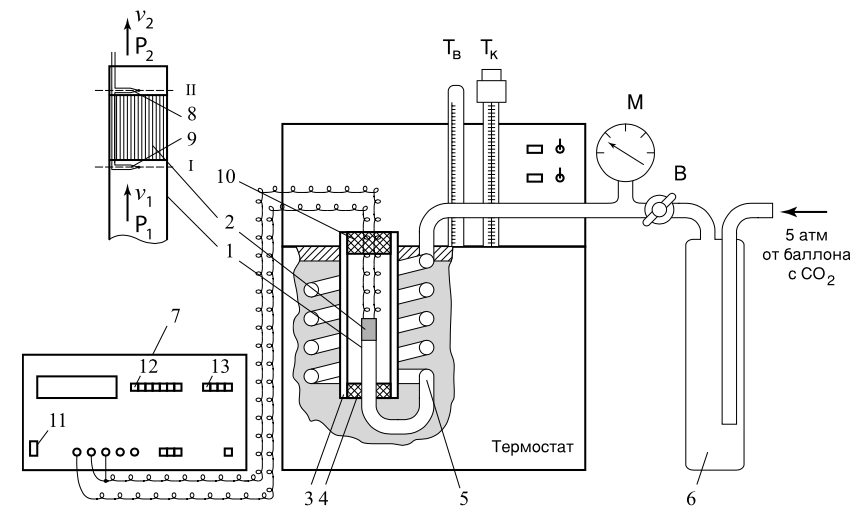
\includegraphics[scale = 0.5]{./stand.png}
	\caption{Схема установки}
	\label{fig:stand}
\end{figure}

Величина эффекта Джоуля–Томсона определяется по разности температуры газа до и после перегородки.

Рассмотрим стационарный поток газа, проходящего через перегородку. 
Чтобы заполнить трубку газом до перегородки необходимо совершить 
работу $A_1 = P_1 V_1$, газ проходя через перегородку совершит работу 
$A_2 = P_2 V_2$.
Обмена энергией с окружающей средой не происходит, поэтому:
\begin{equation} \label{eq:delta-work}
A_1 - A_2 = \left(U_2 + \dfrac{\mu v_2^2}{2}\right) - \left(
U_1 + \dfrac{\mu v_1^2}{2} \right).
\end{equation}

После некоторых преобразований:
\begin{equation} \label{eq:delta-entalpy}
H_1 - H_2 = \mu \dfrac{v_2^2 - v_1^2}{2}.
\end{equation}

Эффект Джоуля-Томсона наблюдается, если $H_1 - H_2 \approx 0$.
В нашем случае это так, потому что $\Delta T = \dfrac{\mu}{2 C_p} \left( v_2^2 - v_1^2 \right)$ много меньше температуры газа.

Эффект Джоуля-Томсона выражается формулой:
\begin{equation} \label{eq:jt-effect}
\mu_{\tiny{\text{Д-Т}}} = \dfrac{\Delta T}{\Delta P} \approx \dfrac{
	\left( \dfrac{2a}{RT} - b \right)
}{C_p}.
\end{equation}
\section{Приборы и материалы}

В работе используются:

\begin{itemize}
	\item Трубка с пористой перегородкой;
	\item Труба Дьюара;
	\item Термостат;
	\item Термометры;
	\item Дифференциальная термопара;
	\item Микровольтметр;
	\item Балластный баллон;
	\item Манометр.
\end{itemize}

\begin{table}[!htb]
	\centering
	\begin{tabular}{|c|c|c|c|c|c|c|}
		\hline
		Температура, $^{\circ} \text{C}$ &  
		0-10 & 10-20 & 20-30 & 30-40 & 40-50 & 50-60 \\
		\hline
		Чувствительность, $\mu \text{V} / ^{\circ} \text{C}$ &
		38.9 & 39.8 & 40.7 & 41.6 & 42.5 & 43.3 \\
		\hline
	\end{tabular}
	\caption{Чувствительность термопары при различных температурах}
	\label{tab:termopair-ratios}
\end{table}

\section{Обработка результатов}

Запишем полученные в ходе трёх экспериментов результаты в соответствующие таблицы

Погрешность измерения напряжения будем полагать $0.001\text{mV}$, а погрешность давления примем равной половине ЦД.

Измерения при температуре $T_1 = 20^{\circ}~\text{C}$.
$V_0 = 0.006 \text{mV}$.
Чувствительность термопары -- 
$40.25 \mu \text{V} / ^{\circ} \text{C}$
\begin{table}[H]
	\centering
	\begin{tabular}{|c|c|c|c|}
		\hline
		$\Delta P,~\text{атм}$ & $\widetilde{V},~\text{mV}$ & 
		$V,~\text{mV}$ & $\Delta T,~^{\circ}\text{C}$ \\
		\hline
		4.2 & 0.176 & 0.170 & 4.37 \\
		3.9 & 0.160 & 0.164 & 3.98 \\
		3.6 & 0.145 & 0.139 & 3.60 \\
		3.3 & 0.131 & 0.125 & 3.25 \\
		3.0 & 0.117 & 0.111 & 2.91 \\
		\hline
	\end{tabular}
\end{table}

Измерения при температуре $T_2 = 30^{\circ}~\text{C}$.
$V_0 = 0.002 \text{mV}$.
Чувствительность термопары -- 
$41.15 \mu \text{V} / ^{\circ} \text{C}$
\begin{table}[H]
	\centering
	\begin{tabular}{|c|c|c|c|}
		\hline
		$\Delta P,~\text{атм}$ & $\widetilde{V},~\text{mV}$ & 
		$V,~\text{mV}$ & $\Delta T,~^{\circ}\text{C}$ \\
		\hline
		4.2 & 0.167 & 0.165 & 4.06 \\
		3.9 & 0.151 & 0.149 & 3.67 \\
		3.6 & 0.135 & 0.133 & 3.29 \\
		3.3 & 0.120 & 0.118 & 2.92 \\
		3.0 & 0.107 & 0.105 & 2.60 \\
		\hline
	\end{tabular}
\end{table}

Измерения при температуре $T_3 = 50^{\circ}~\text{C}$.
$V_0 = -0.001 \text{mV}$.
Чувствительность термопары -- 
$42.9 \mu \text{V} / ^{\circ} \text{C}$.
\begin{table}[H]
	\centering
	\begin{tabular}{|c|c|c|c|}
		\hline
		$\Delta P,~\text{атм}$ & $\widetilde{V},~\text{mV}$ & 
		$V,~\text{mV}$ & $\Delta T,~^{\circ}\text{C}$ \\
		\hline
		4.2 & 0.154 & 0.155 & 3.59 \\
		3.9 & 0.135 & 0.136 & 3.15 \\
		3.6 & 0.122 & 0.123 & 2.84 \\
		3.3 & 0.106 & 0.107 & 2.47 \\
		3.0 & 0.095 & 0.096 & 2.21 \\
		\hline
	\end{tabular}
\end{table}

По полученным значениям построим графики. По графикам найдем коэффициент Джоуля-Томсона, его погрешность определим как корень из суммы квадратов отклонений.

\[
	\Delta \mu = \sqrt{\frac{1}{5}\sum_{i=1}^5 (\mu_i - <\mu>)^2}
\]

\begin{figure}[H]
	\centering
	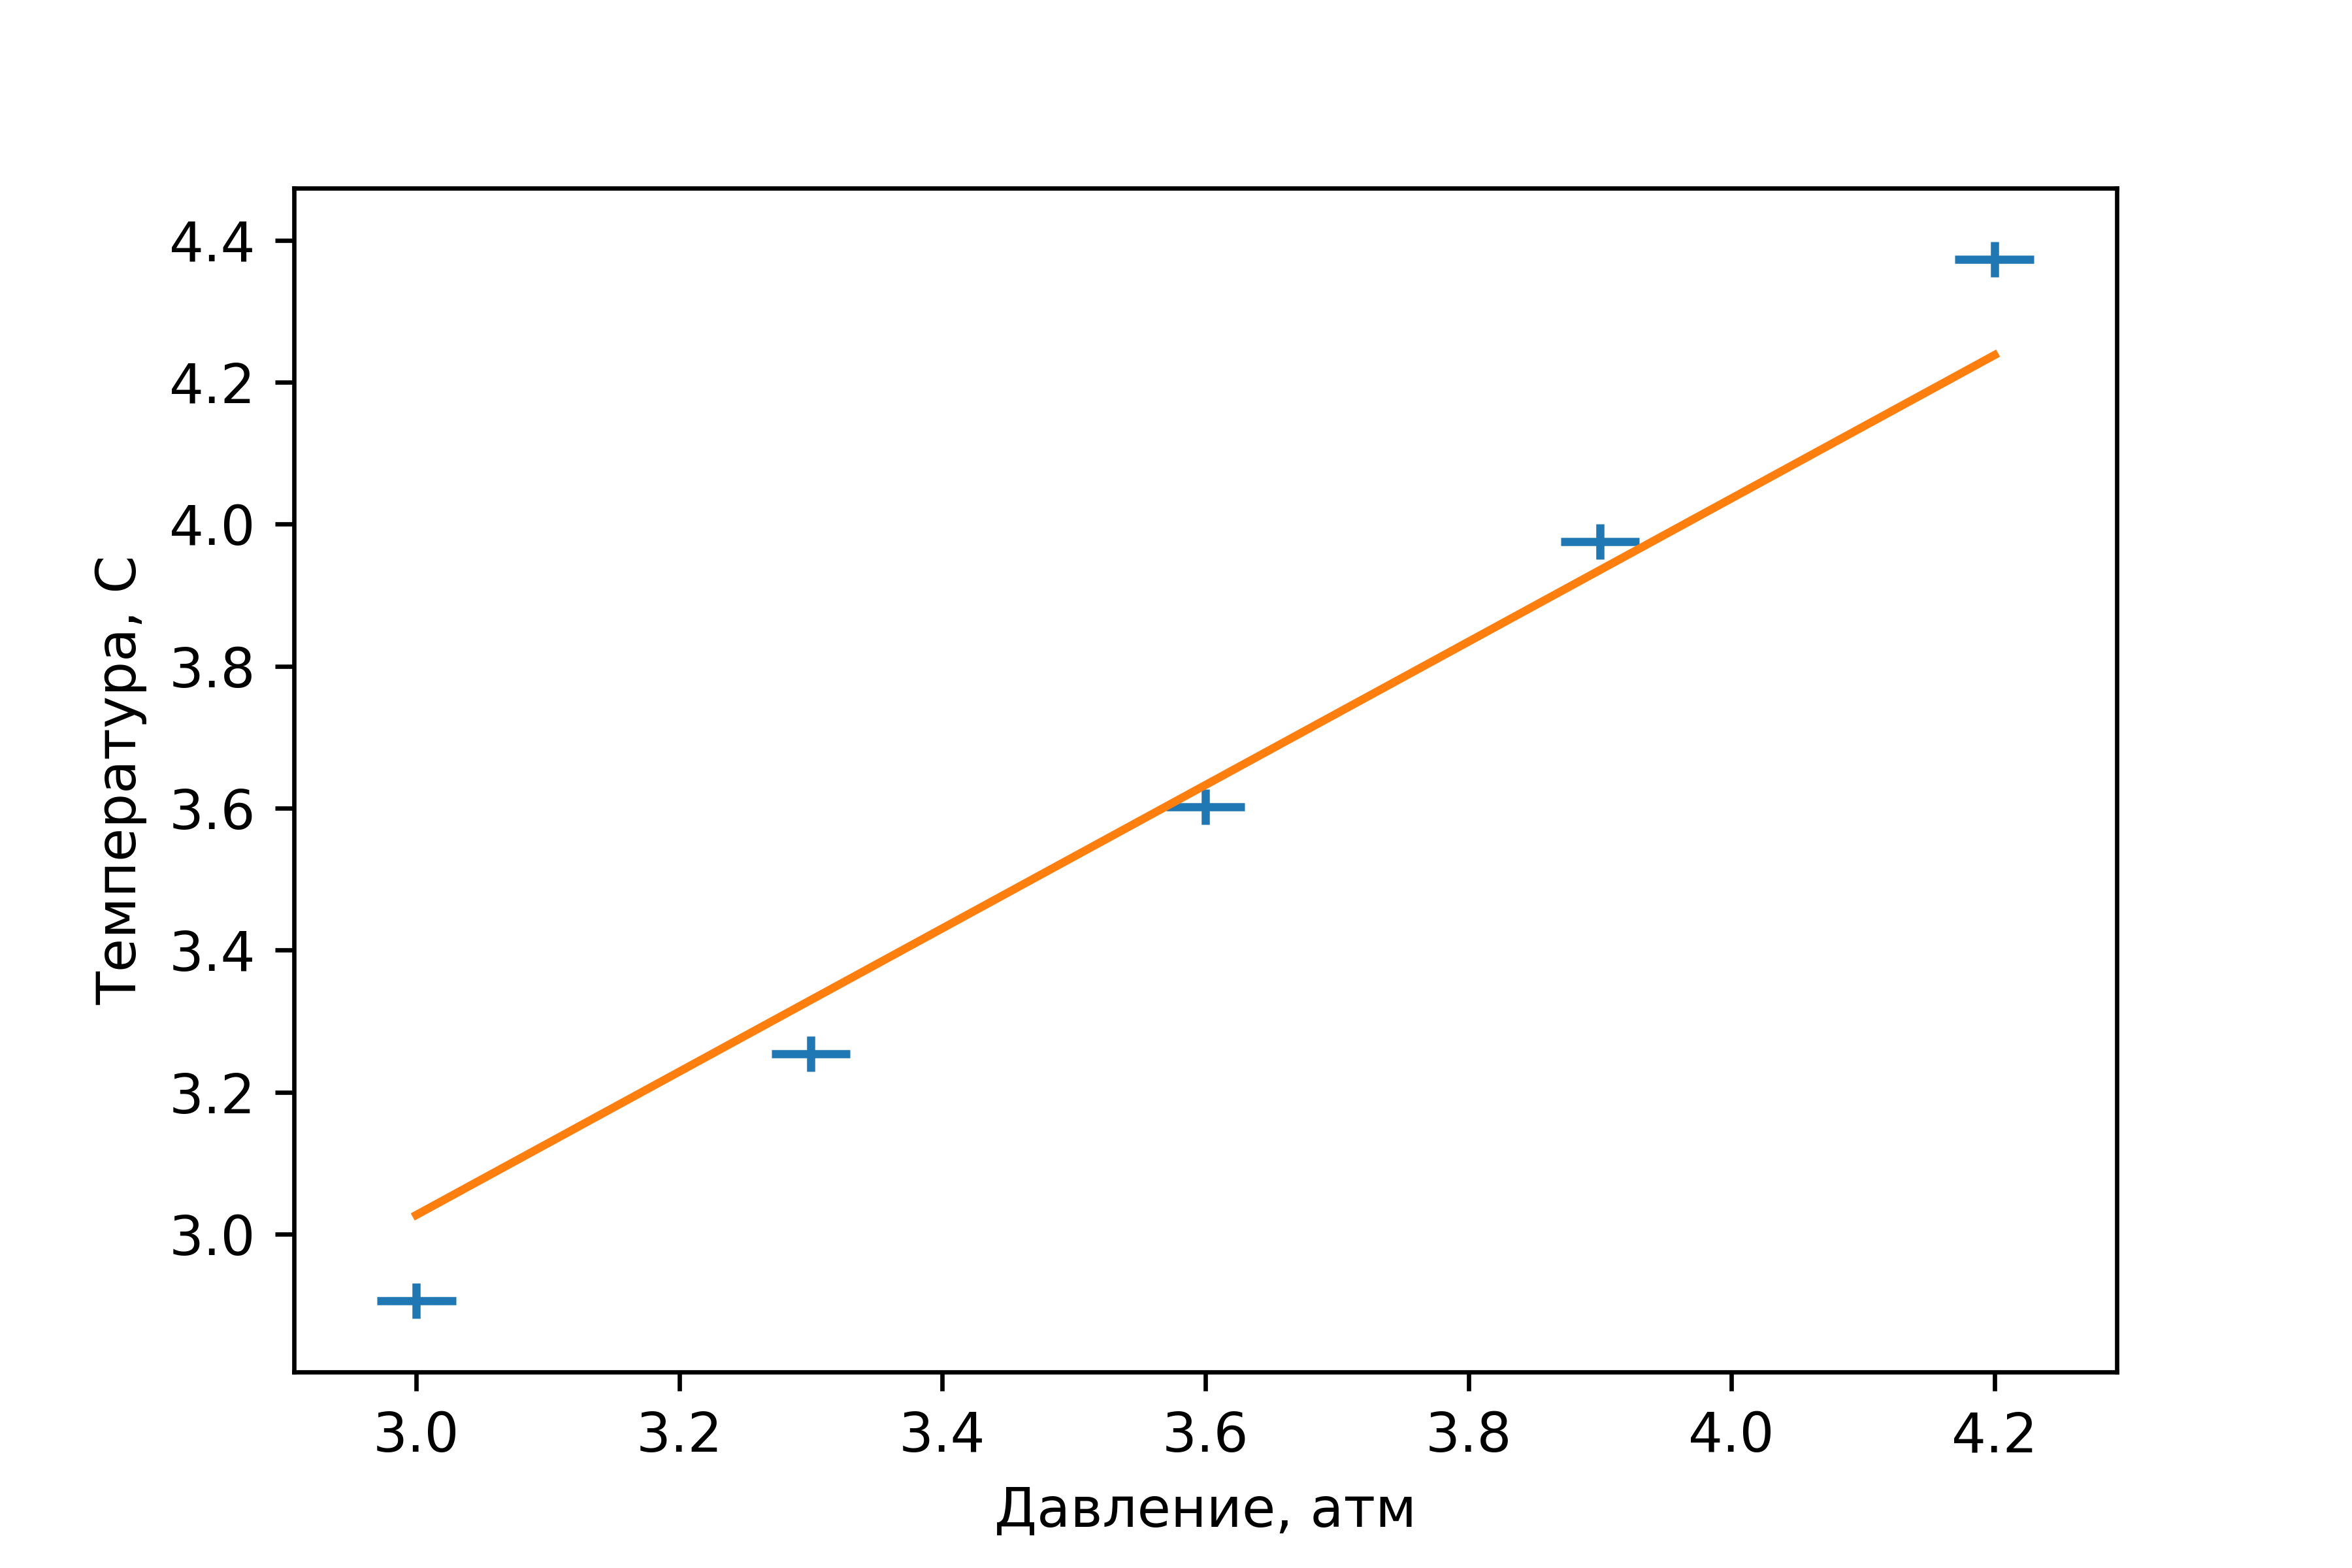
\includegraphics[width=0.8\textwidth]{./data-20.png}
	\caption{
		График $\Delta T \left( \Delta p \right)$ 
		для $T=20^{\circ} \text{C}$.
		$\mu_{\tiny{\text{Д-Т}}} = 1.01 \pm 0.03 \dfrac{K}{\text{атм}}$
	}
\end{figure}

\begin{figure}[H]
	\centering
	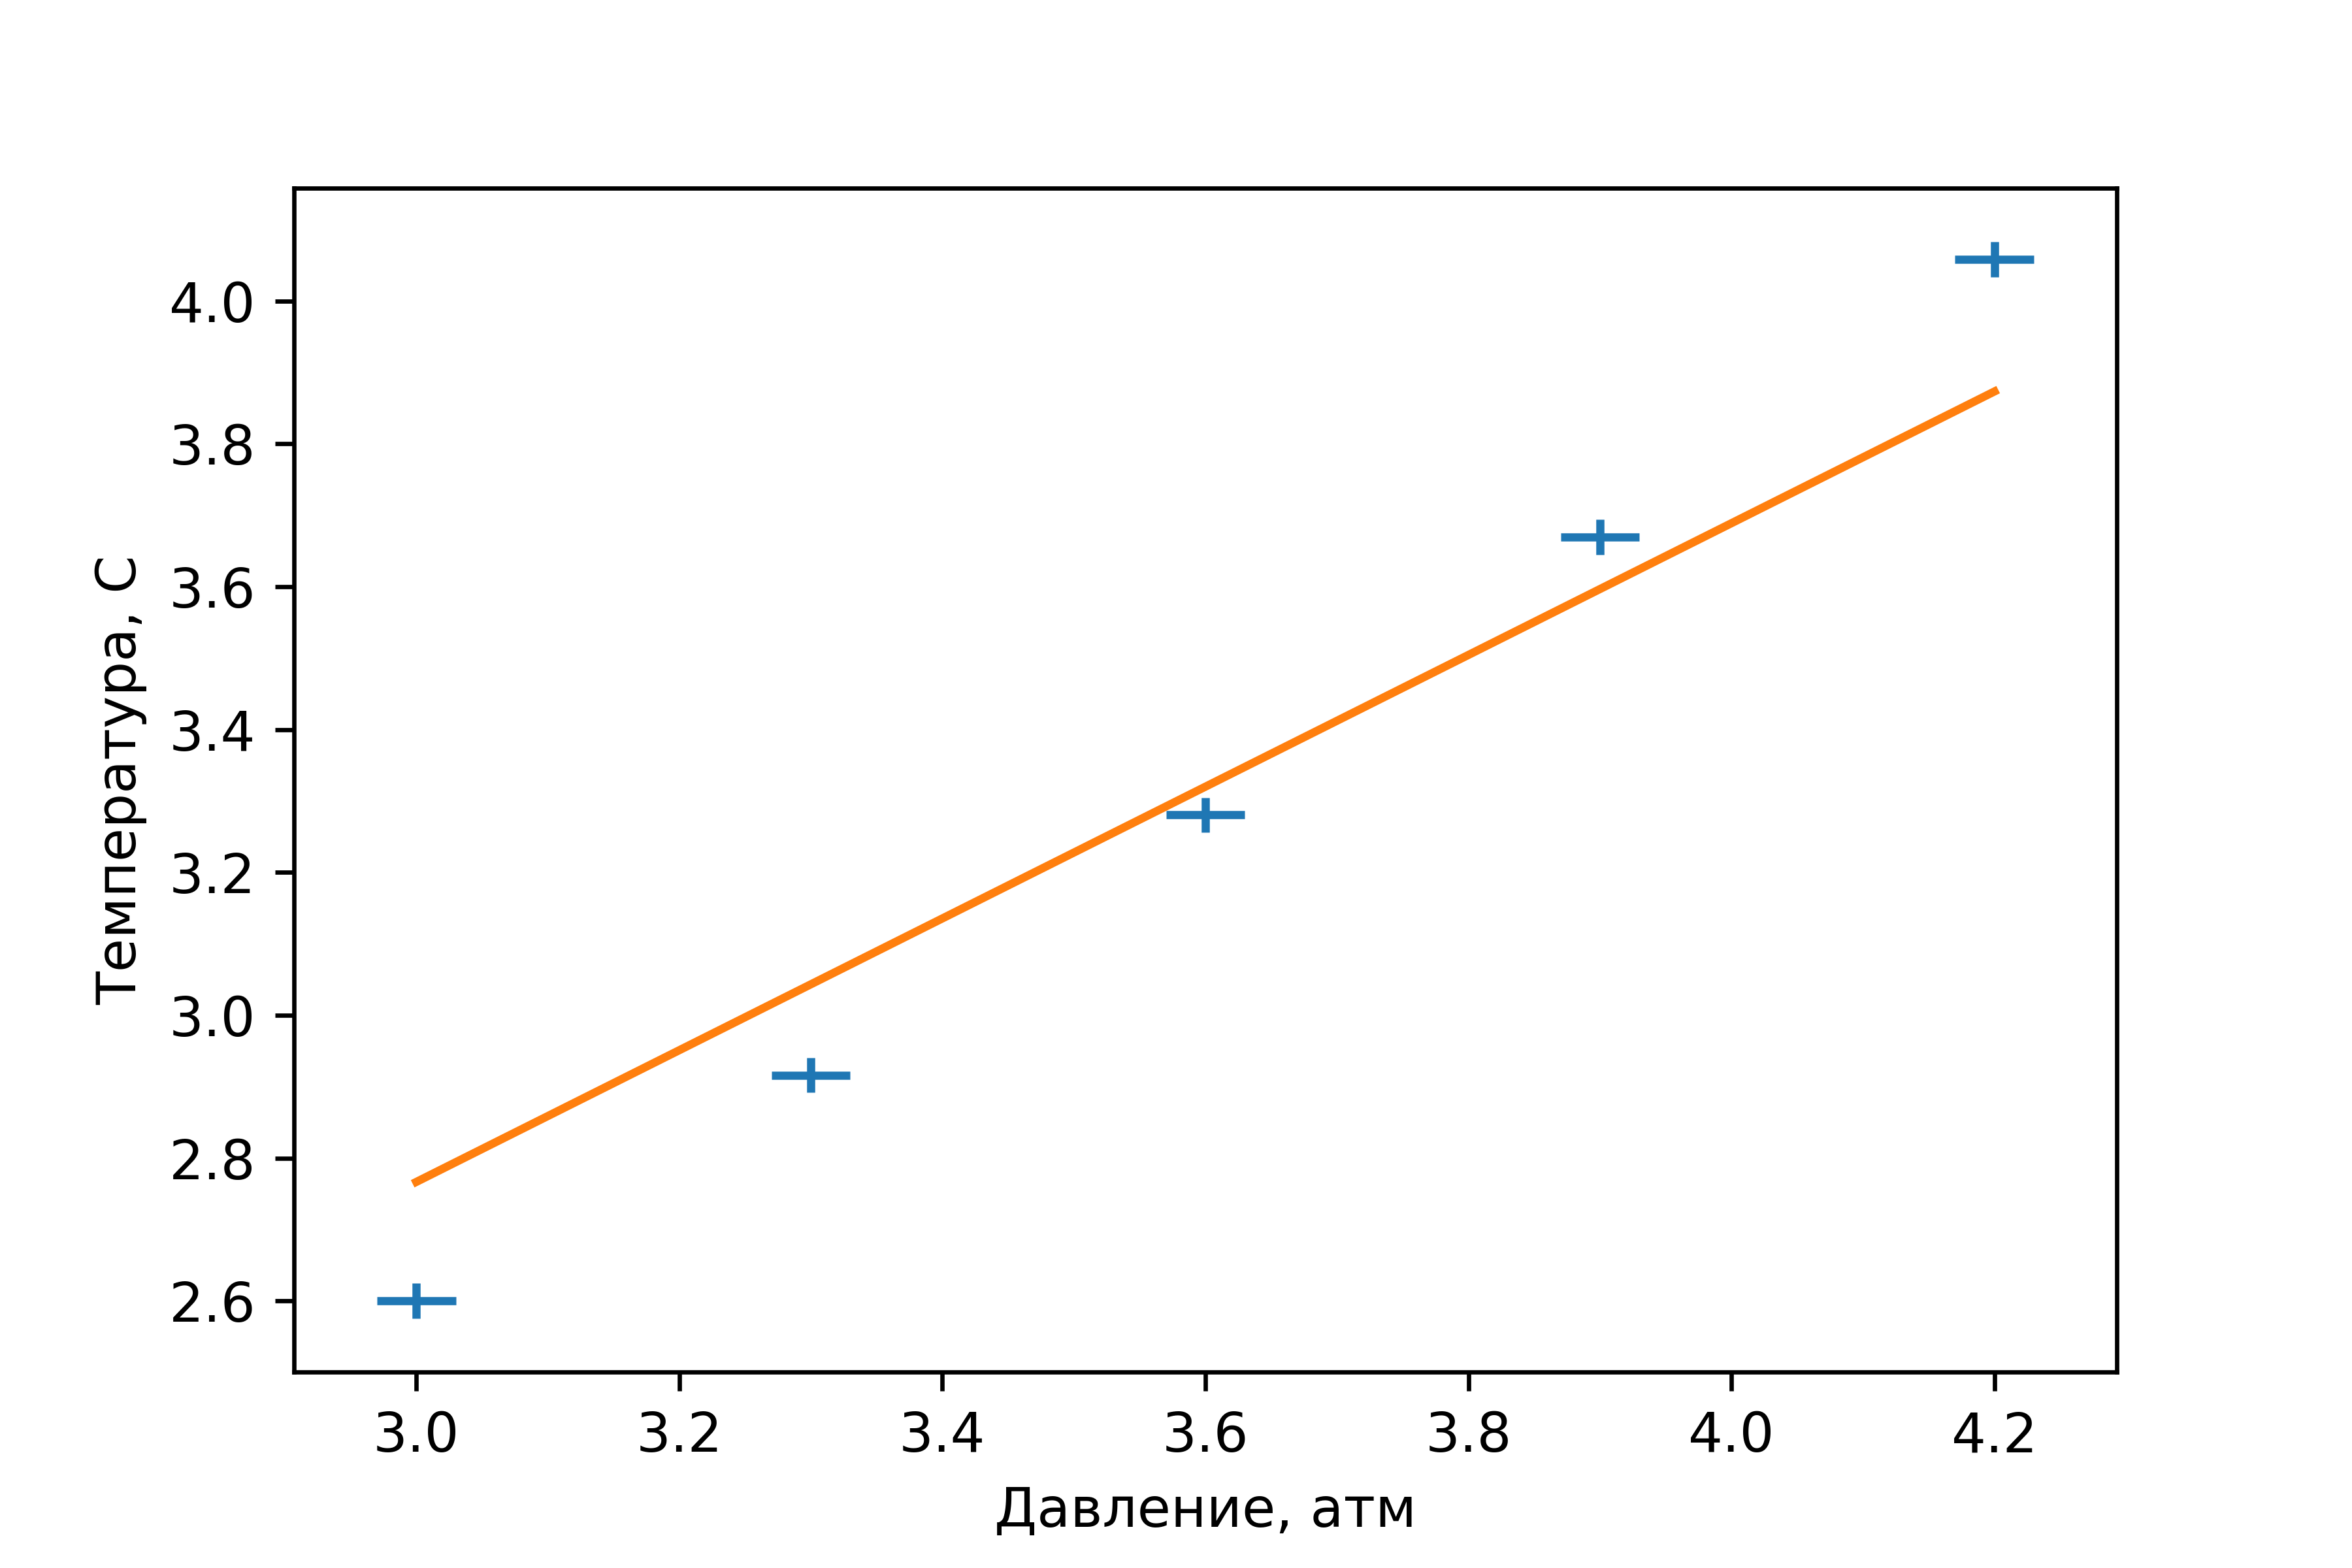
\includegraphics[width=0.8\textwidth]{./data-30.png}
	\caption{
		График $\Delta T \left( \Delta p \right)$ 
		для $T=30^{\circ} \text{C}$.
		$\mu_{\tiny{\text{Д-Т}}} = 0.92 \pm 0.04 \dfrac{K}{\text{атм}}$
	}
\end{figure}

\begin{figure}[H]
	\centering
	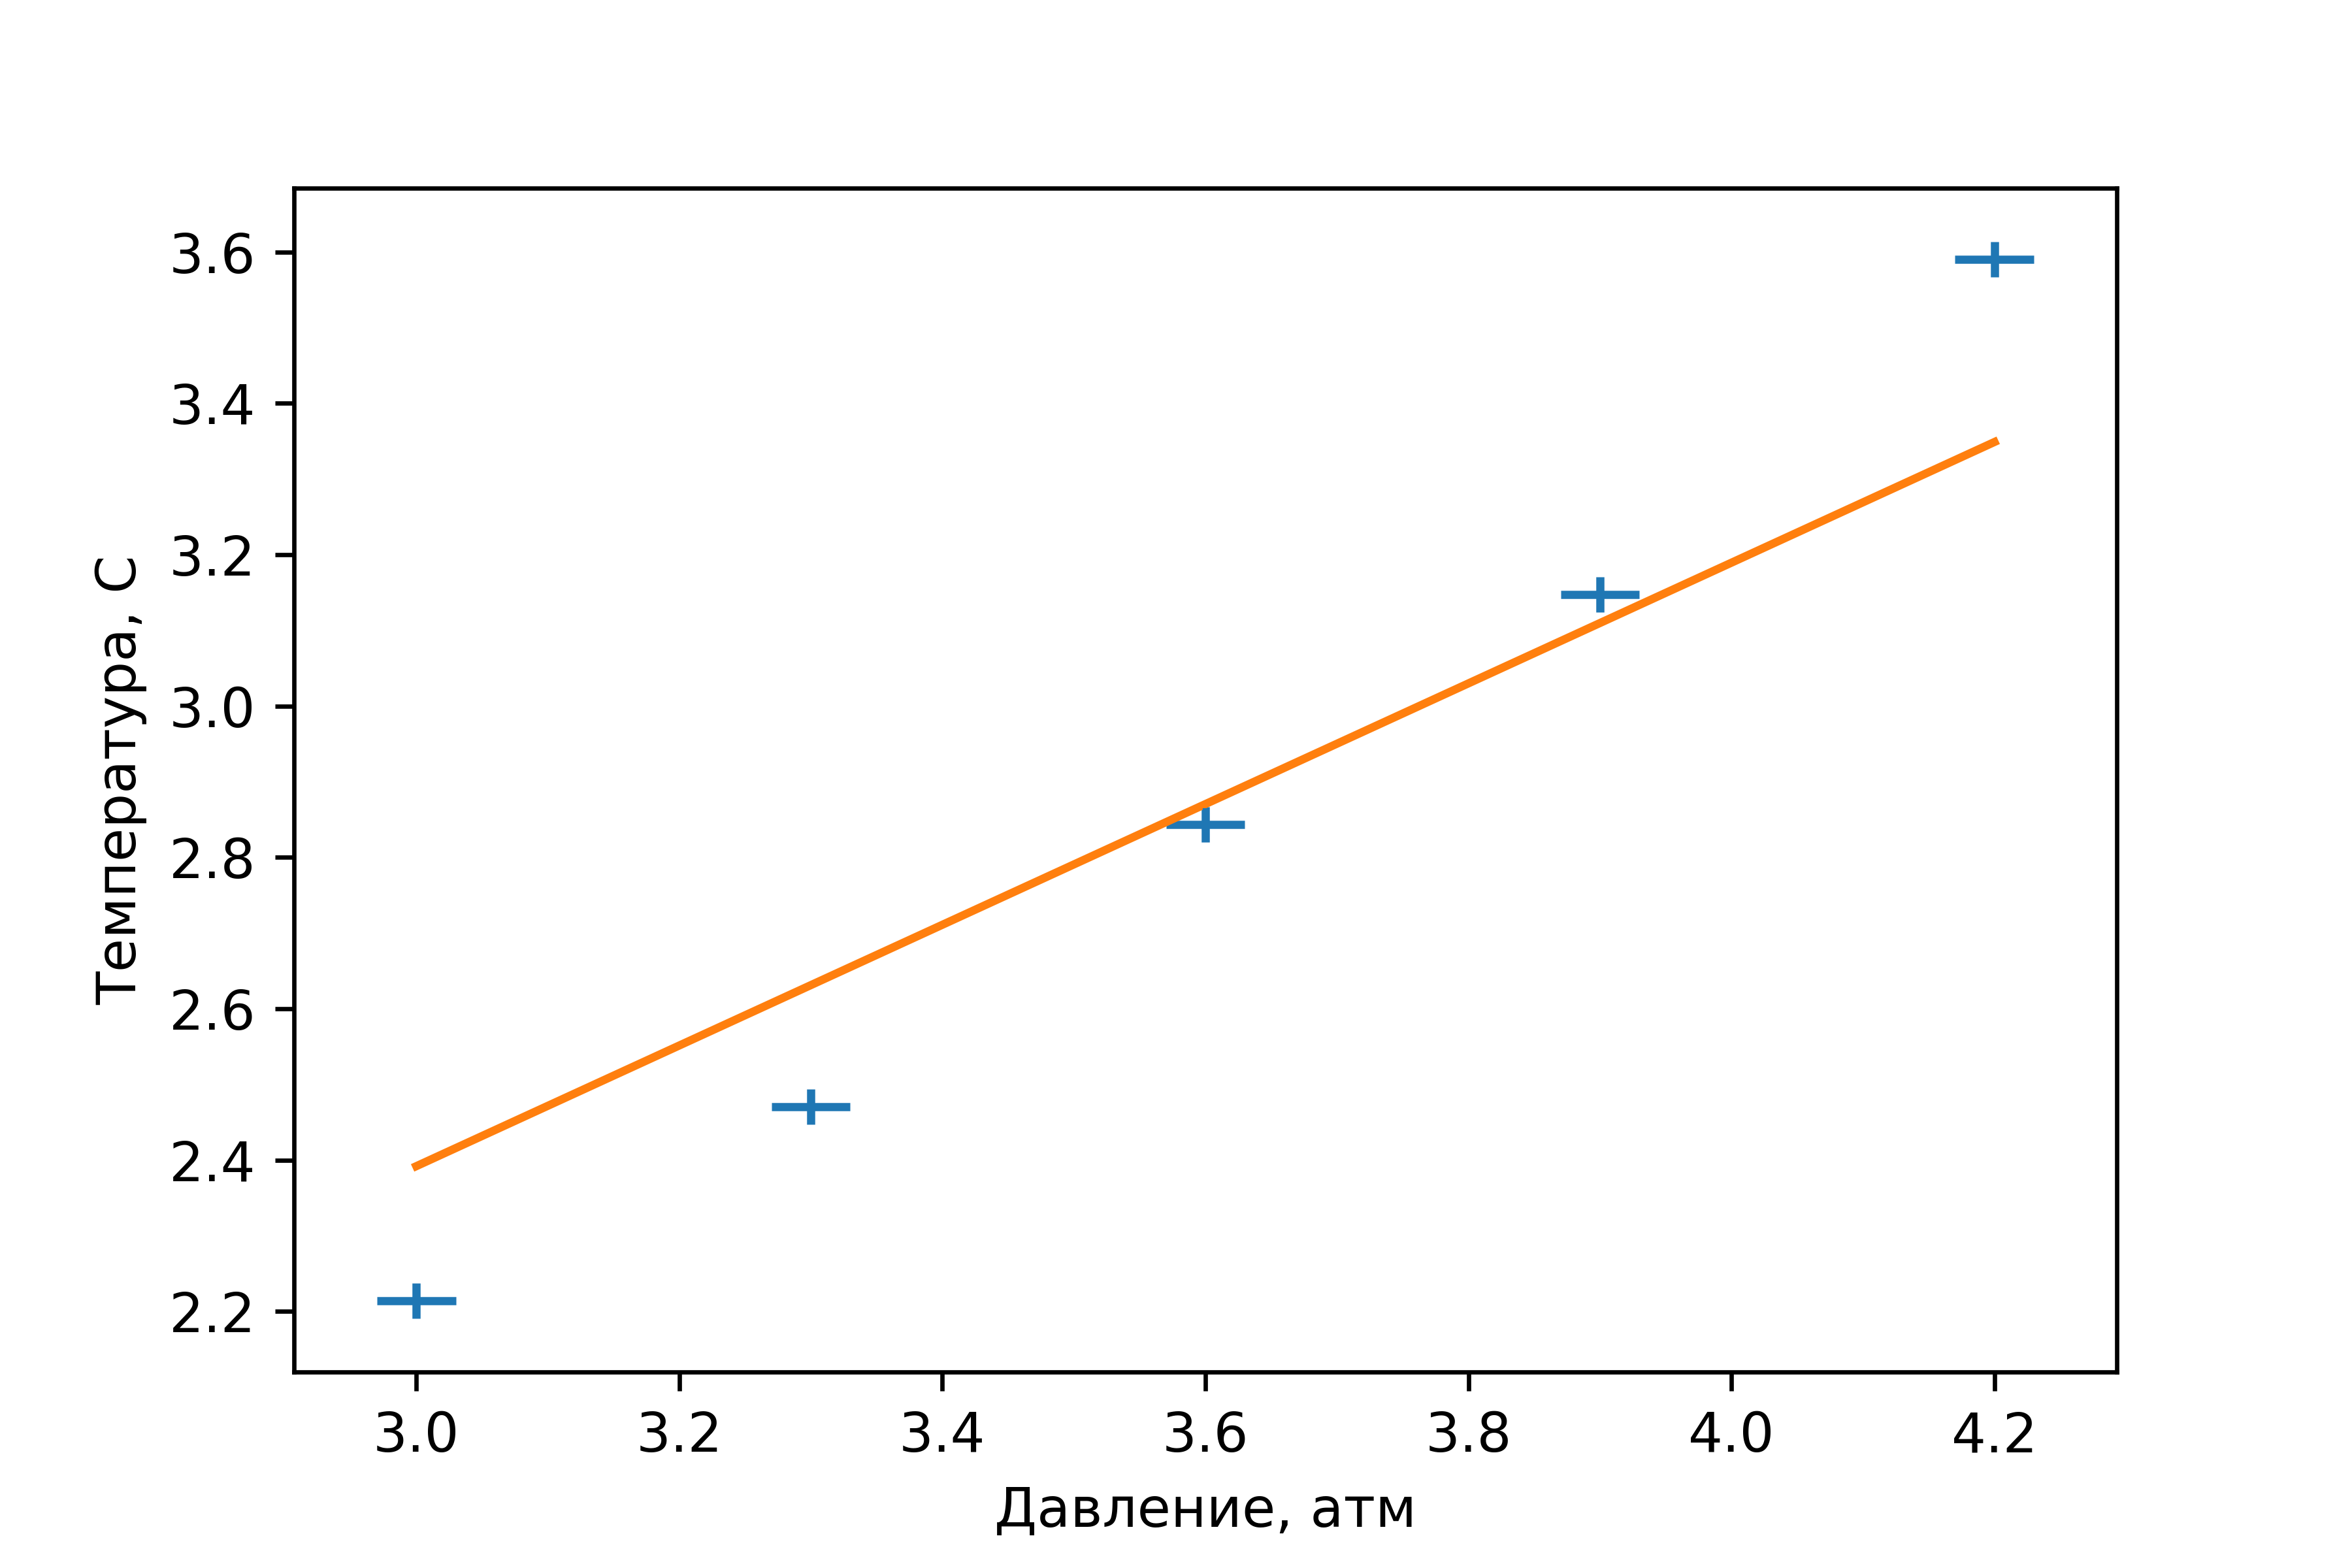
\includegraphics[width=0.8\textwidth]{./data-50.png}
	\caption{
		График $\Delta T \left( \Delta p \right)$ 
		для $T=50^{\circ} \text{C}$.
		$\mu_{\tiny{\text{Д-Т}}} = 0.80 \pm 0.04 \dfrac{K}{\text{атм}}$
	}
\end{figure}

Составим систему:
\begin{equation} \label{eq:van-der-vaals-parameters}
\begin{cases}
\dfrac{
	\left( \dfrac{2a}{RT_1} - b \right)
}{C_p} = \mu_1 \\
\dfrac{
	\left( \dfrac{2a}{RT_2} - b \right)
}{C_p} = \mu_2 \\
\dfrac{
	\left( \dfrac{2a}{RT_3} - b \right)
}{C_p} = \mu_3 \\
\end{cases}.
\end{equation}

Для каждой пары уравнений можно найти соответствующие $a$ и $b$.
Решим систему и запишем результаты в таблицу:
\begin{table}[H]
	\centering
	\begin{tabular}{|c|c|}
		\hline
		$a, \text{м}^3 \cdot \text{Па}$ & $b, 10^{-4}~\text{м}^3$ \\
		\hline
		0.97 & 4.99 \\
		\hline
		0.71 & 2.97 \\
		\hline
		0.80 & 3.64 \\
		\hline
		$<a>, \text{м}^3 \cdot \text{Па}$ & 
		$<b>, 10^{-4}~\text{м}^3$ \\
		\hline
		0.83 & 3.87 \\
		\hline
	\end{tabular}
	\caption{Значения параметров в уравнении Ван-Дер-Ваальса}
	\label{tab:van-der-vaals-params}
\end{table}

Зная параметры из уравнения Ван-дер-Ваальса, рассчитаем температуру инверсии
\begin{equation} \label{eq:inverse-temperature}
T_{inv} = \dfrac{2a}{Rb} \approx 516 \text{К}.
\end{equation}

Найдем погрешность измерения параметров $a$ и $b$, а так же температуры инверсии.
\begin{align*}
& \mu_{\tiny{\text{Д-Т}}} = \dfrac{\dfrac{2a}{RT} - b}{c_p} \\
& \left( \mu_1 - \mu_2 \right) c_p = \dfrac{2a}{R} \left( 
\dfrac{1}{T_1} - \dfrac{1}{T_2}
\right) 
\end{align*}

\begin{equation*} \label{eq:delta_a}
 a = \dfrac{R c_p \left( \mu_1 - \mu_2 \right)}{2 \left(
	\dfrac{1}{T_1} - \dfrac{1}{T_2}
	\right)} \\
\end{equation*}

\begin{multline*}
\Delta a  = \sqrt{
	\left( \dfrac{\partial a}{\partial \mu_1} \right)^2 
	\cdot \Delta \mu_1^2 +
	\left( \dfrac{\partial a}{\partial \mu_2} \right)^2 
	\cdot \Delta \mu_2^2 +
	\left( \dfrac{\partial a}{\partial T_1} \right)^2 
	\cdot \Delta T_1^2 +
	\left( \dfrac{\partial a}{\partial T_2} \right)^2 
	\cdot \Delta T_2^2
} \\
 = \sqrt{
	2 \left( 
	\dfrac{R c_p}{2 \left( T_1^{-1} + T_2^{-1} \right)} 
	\right)^2 \Delta \mu^2 +
	2 \left(
	\dfrac{R c_p \left( T_1^2 + T_2^2 \right)}
	{2 \left( T_1 + T_2 \right)^2}
	\right)^2 \Delta T^2
} \approx 0.1 \text{м}^3 \cdot \text{Па}
\end{multline*}

\begin{equation*}
 b = \dfrac{2a}{RT} - \mu_{jt} c_p 
\end{equation*}

\begin{multline*}
 \Delta b = \sqrt{
	\left( \dfrac{\partial b}{\partial \mu} \right)^2 
	\Delta \mu^2 +
	\left( \dfrac{\partial b}{\partial T} \right)^2 \Delta T^2 +
	\left( \dfrac{\partial b}{\partial a} \right)^2 \Delta a^2
} = \\
 = \sqrt{
	c_p^2 \Delta \mu^2 + 
	\left( \dfrac{2a}{RT^2} \right)^2 \Delta T^2 +
	\left( \dfrac{2}{RT} \right)^2 \Delta a^2
} \approx 0.8 \cdot 10^{-4} \text{м}^3
\end{multline*}

\begin{align*}
& T_{inv} = \dfrac{2a}{Rb} \\
& \Delta T_{inv} = T_{inv} \sqrt{
	\left( \dfrac{\Delta a}{a} \right)^2 +
	\left( \dfrac{\Delta b}{b} \right)^2
} = 123.5 ^{\circ} C
\end{align*}

\section{Вывод}

По результатам эксперимента удалось определить коэффициенты уравнения Ван-дер-Ваальса $a = (0.8 \pm 0.1)\text{Па} \cdot\text{м}^3$ и $b = (3.87\pm 0.8)\cdot 10^{-4} \text{м}^3$, а так же температуру инверсии углекислого газа $T_{inv} = (516 \pm 123.5)^{\circ}C$.  Видно, что результаты весьма сильно разнятся с табличными $a = 0.36 \text{Па} \cdot \text{м}^3$, $b = 4.284 \cdot 10^{-4} \text{м}^3$, $T_{inv} = 2050 \text{К}$. Это может быть обусловлено как малым количеством измерений в каждом эксперименте, так и тем фактом, что уравнение Ван-дер-Ваальса не позволяет с достаточной точностью описать поведение реального газа.

\end{document}